\documentclass[11pt,a4paper]{article}
\usepackage{fontspec}
\usepackage{polyglossia}
\setmainlanguage{ukrainian}
\setotherlanguage{english}
\setmainfont{cmunrm.otf}[Path=fonts/,BoldFont=cmunbx.otf,ItalicFont=cmunti.otf,BoldItalicFont=cmunbi.otf]
\setsansfont{cmunss.otf}[Path=fonts/,BoldFont=cmunsx.otf,ItalicFont=cmunsi.otf,BoldItalicFont=cmunso.otf]
\setmonofont{cmuntt.otf}[Path=fonts/,ItalicFont=cmunit.otf]
\newfontfamily\cyrillicfont{cmunrm.otf}[Path=fonts/,BoldFont=cmunbx.otf,ItalicFont=cmunti.otf,BoldItalicFont=cmunbi.otf,Script=Cyrillic]
\newfontfamily\cyrillicfontsf{cmunss.otf}[Path=fonts/,BoldFont=cmunsx.otf,ItalicFont=cmunsi.otf,BoldItalicFont=cmunso.otf,Script=Cyrillic]
\newfontfamily\cyrillicfonttt{cmuntt.otf}[Path=fonts/,ItalicFont=cmunit.otf,Script=Cyrillic]
\usepackage[a4paper,margin=25mm]{geometry}
\usepackage{microtype}
\usepackage{booktabs,longtable,tabularx,array,multirow}
\usepackage{graphicx}
\graphicspath{{../figures_uk/}}
\newcolumntype{Y}{>{\raggedright\arraybackslash}X}
\usepackage{caption}
\captionsetup{font=small,labelfont=bf,labelsep=colon,justification=justified,singlelinecheck=false}
\captionsetup[table]{position=top}
\usepackage{enumitem}
\usepackage{amsmath}
\usepackage{float}
\usepackage[section]{placeins}
\usepackage[numbers,sort&compress]{natbib}
\usepackage{xurl}
\usepackage{hyperref}
\urlstyle{same}
\hypersetup{hidelinks,pdfencoding=auto,unicode=true,pdftitle={Social: доказово обґрунтований фреймворк для автоматизованого аналізу соціальних конфліктів та інформаційних інцидентів},pdfauthor={Oleksandr Pylypenko}}
\emergencystretch=2em
\setlist{nosep,leftmargin=1.5em}
\renewcommand{\arraystretch}{1.12}
\renewcommand{\bibfont}{\small}
\setlength{\bibsep}{2pt}

\DeclareRobustCommand{\code}[1]{\nolinkurl{#1}}
\newcommand{\baseline}{\texttt{f0e9d0d}}
\begin{document}
\begin{center}
{\LARGE Social: доказово обґрунтований фреймворк для автоматизованого аналізу соціальних конфліктів та інформаційних інцидентів\par}
\vspace{0.4em}
{\large Архітектура, реалізація, оцінювання та уроки реального кейсу\par}
\vspace{0.8em}
{\large Олександр Пилипенко\par}
{\small Незалежний дослідник у галузі штучного інтелекту та машинного навчання\par}
{\small Аспірант, Державний торговельно-економічний університет, Київ, Україна\par}
{\small ORCID: \href{https://orcid.org/0009-0004-9610-9242}{0009-0004-9610-9242}\par}
{\small \href{mailto:O.Pylypenko@knute.edu.ua}{\texttt{O.Pylypenko@knute.edu.ua}}\par}
\vspace{0.4em}
10 листопада 2026 р. \textperiodcentered{} Версія 1.1\par
{\small Українська редакція. Основною є англомовна редакція того самого дослідження.\par}
\end{center}
\begin{abstract}
Цифрові сліди соціальних конфліктів поєднують неповні спостереження, повторювані твердження, суперечливі свідчення та медіа, час публікації яких відрізняється від часу запису чи події. Інтеграція цих записів потребує автоматизації, яка зберігає межі доказовості, а не генерує єдину впевнену оповідь. У статті описано Social --- модульну дослідницьку систему на Python, що поєднує збір даних окремо за платформами, версіоновані знімки, аналіз схожості текстів і часу, облік доказів, обмежений пошук, типізоване впорядкування подій, локальну обробку медіа та контрольні перевірки звітів. Проведено аудит зафіксованої реалізації та розмежовано реалізовані функції, структурні тести, емпіричні перевірки й невиміряні семантичні властивості. Оцінювання відтворює вичерпний граф текстової схожості між каналами із 369 ребер, знаходить 367 із них у результатах застарілого MinHash, повторно обчислює 16 збережених підсумків умовної рандомізації та відтворює префікс із 25 вибірок для кожної з чотирьох нульових моделей. Свіжий офлайн-набір проходить 783 тести й 16 підтестів. Ці результати встановлюють обмежену обчислювальну відтворюваність, а не фактичну точність. Поточний кураторський пакет із 25 тверджень видає 19 станів «підтримано в межах обсягу» та шість станів «недостатньо доказів», проте цільові випробування виявляють помилки числових присудків і заперечень в евристиках відношень. Оприлюднена післяаудитна ревізія правила усуває всі 36 прийнять хибного присудка й заперечення в авторському стрес-тесті на 534 випадки та змінює результат пакета на 18 підтриманих і сім із недостатніми доказами; цей стрес-тест не є оцінкою точності. Загальний офлайн-процес консервативно зберігає знайдені твердження неперевіреними й потребує окремо наданих входів звіту. Історичні медіаквитанції документують 607 декодованих активів; порівняння 18 кліпів із наданим еталоном дає micro-WER 44,58\% без незалежно встановленого походження перевірки еталона. Реальний кейс ілюструє інтеграцію та обмеження охоплення. Внесок Social --- придатний для перегляду аналітичний процес і явний опис меж його надійності, а не новий алгоритм висновування чи валідований автономний дослідник.
\end{abstract}
\noindent\textbf{Ключові слова:} обчислювальна соціальна наука; кризова інформатика; походження доказів; автоматизований аналіз; інформаційна динаміка; дослідницьке програмне забезпечення; невизначеність.

\section{Вступ}
Соціальні конфлікти дедалі частіше залишають паралельні записи в каналах, гілках коментарів, новинних повідомленнях, заявах установ і коротких аудіовізуальних фрагментах. Ці записи слугують різним аналітичним завданням: зафіксувати, що сказало джерело, простежити поширення твердження, виявити повторений текст, упорядкувати можливі події та оцінити, чи підтримують наявні докази певне звинувачення. Система, яка змішує ці завдання, може перетворити правдоподібну оповідь на нібито перевірений опис. Скопійоване твердження не є новим свідком, час публікації не є часом запису, а статистичне відхилення від моделі часу не вказує на організатора.

Кризова інформатика давно наголошує на складності отримання корисної інформації з неоднорідних і зашумлених потоків соціальних мереж \citep{imran2015crisis}. Обчислювальна соціальна наука додає питання доступу до платформ, вибірки, вимірювання та етики \citep{Olteanu2019,VicentePaula2023}. Цифрове розслідування за відкритими джерелами потребує збереження й контекстуальної перевірки матеріалів, зокрема явного опису невизначеності \citep{berkeleyProtocol2022}. Ці вимоги стають особливо важливими, коли програмне забезпечення поєднує традиційний аналіз із генеративним ШІ. Вправний синтез може приховувати невизначеність, а не усувати її; навіть генерація з цитуванням потребує окремої оцінки того, чи підтримують цитати сам текст \citep{gao2023alce}.

Social розв'язує цю інтеграційну проблему як дослідницький програмний фреймворк. Його практична мета --- допомогти аналітику перейти від зібраних цифрових слідів до придатних для перегляду проміжних записів та обмежених аналітичних результатів. Реалізація містить скрипти отримання даних для окремих платформ, аналіз інформаційних хвиль, зв'язаний реєстр доказів, правила пошуку й перевірки, обробку типізованих подій, локальні медіаконвеєри та валідатори звітів. Ці компоненти суттєво різняться за зрілістю, інтегрованістю й оціненістю. Опис їх як єдиного рівномірно автономного дослідника приховав би ці відмінності.

Стаття ставить питання: \emph{як модульна, доказово обґрунтована програмна система може інтегрувати неоднорідні цифрові сліди для автоматизованого аналізу соціальних конфліктів та інформаційних інцидентів, зберігаючи походження даних, невизначеність і відтворюваність?} Ми вивчаємо наявну реалізацію, а не пропонуємо новий алгоритм. Аналіз фіксує ревізію Git, досліджує шляхи виконання, звіряє числові артефакти, повторно запускає обмежені обчислення й навмисно перевіряє випадки семантичних збоїв. Кейс Петропавлівської Борщагівки дає реалістичні робочі навантаження, але не є незалежною перевіркою узагальнюваності. Сам інцидент вивчено в окремому рукописі проєкту \citep{pylypenko2026case}; ця стаття розглядає програмне забезпечення та межі його доказовості.

\subsection{Внесок роботи}
Внесок роботи складається з чотирьох частин. По-перше, подано інтеграційну карту, засновану на коді, яка розмежовує повторно використовувані процесори, збирачі платформ, експериментальні евристики, кураторські збирачі кейсу та скрипти формування звітів. По-друге, описано реалізовану модель доказів і розрізнення технічного походження, лінії походження інформації, незалежності джерел та семантичної обґрунтованості. По-третє, наведено перевірки відтворюваності для виявлення схожості, умовної рандомізації, структурних контрактів та обмеженого офлайн-процесу. По-четверте, показано конкретні семантичні контрприклади, виміряно на них оприлюднену ревізію правила й визначено межі продемонстрованої автономності системи. Цей внесок сприяє відповідальнішому використанню й оцінюванню аналітичного програмного забезпечення, але не встановлює нового рівня техніки у перевірці фактів, виділенні подій чи атрибуції.

\section{Споріднені роботи}
\label{sec:related}

Social перебуває на перетині кризової інформатики, баз даних новинних подій, автоматизованої перевірки тверджень, генерації з опорою на пошук і практики цифрових розслідувань. Ці напрями працюють із різними одиницями: повідомленнями, зафіксованими подіями, твердженнями, відповідями або збереженими медіа. Тому їхні результати потребують різної валідації. Знайдена стаття може бути релевантною, але не підтримувати твердження; кілька повідомлень можуть мати одне походження; а декодоване відео може лишатися неперевіреним щодо місця, часу чи тлумачення. Це розрізнення використано для позиціювання дослідженого програмного забезпечення, а не для трактування суміжних систем як взаємозамінних конкурентів. У таблиці~\ref{tab:related} підсумовано їхні задокументовані призначення та межі порівняння.

Безпосередню постановку проблеми дає кризова інформатика. Імран та співавтори~\cite{imran2015crisis} організовують обробку екстрених повідомлень навколо фільтрації, класифікації, ранжування, агрегації, виділення та реферування. Така рамка пов'язує неоднорідний збір із потребою аналітика зменшити інформаційне перевантаження. Social використовує подібний погляд на робочий процес, але досліджує обмежену реконструкцію інциденту та придатні для перегляду артефакти. Його панелі платформ і правила добору для конкретного кейсу не становлять репрезентативної вибірки генеральної сукупності. Тому успішне виконання фільтра чи збирача не може встановити повноту, ситуаційну точність або корисність для служб реагування без окремої оцінки цих результатів.

Інфраструктури новинних подій показують, що впорядкування спостережень у події є усталеним завданням. GDELT відокремлює закодовані за CAMEO записи подій від згадок у новинах і надає впевненість виділення та географічні атрибути; його GKG містить сутності, теми й контекстні метадані на рівні документа~\cite{gdelt2015events,gdelt2015gkg}. ACLED спирається на кодування дослідниками та визначену таксономію політичних заворушень із явною точністю дати й місця та інформацією про джерела~\cite{acledCodebook}. Event Registry групує багатомовні новинні статті, виділяє атрибути подій і підтримує їх пошук та дослідження~\cite{leban2014eventregistry}. Ці роботи обґрунтовують явні одиниці подій і розрізнення повідомлень та самих подій. Social не претендує на новизну у виділенні чи кластеризації. Його вужче дослідницьке питання стосується того, як квитанції збору, доказові уривки, оцінки тверджень і гіпотези подій можуть залишатися придатно для перегляду пов'язаними в межах обмеженого розслідування.

Автоматизована перевірка фактів додає доповнювальну вимогу: оцінювати докази так само, як і передбачений висновок. FEVER поєднує твердження, виведені з Wikipedia, із добором доказів і мітками «підтримано», «спростовано» або «недостатньо інформації»~\cite{thorne2018fever}. AVeriTeC працює з твердженнями реального світу, використовуючи вебдокази, декомпозиції запитань і відповідей та обґрунтування, з окремою увагою до часових витоків і достатності доказів~\cite{schlichtkrull2023averitec}. InFact реалізує поетапний конвеєр перевірки фактів на основі пошуку та LLM~\cite{rothermel2024infact}. Це релевантні постановки завдань і прецеденти оцінювання. Контрактні перевірки та регресії Social для інциденту не дорівнюють результату на бенчмарках FEVER чи AVeriTeC, і жодного рейтингу точності щодо цих систем не передбачено. Правильність на рівні тверджень і якість реконструкції лишаються окремими від успіху програмної інтеграції.

Генерація з доповненням пошуком поєднує навчену генерацію із зовнішньою знайденою пам'яттю~\cite{lewis2020rag}. ALCE робить якість цитування окремим виміром оцінювання поряд із правильністю та плавністю~\cite{gao2023alce}. Це розрізнення важливе для згенерованих звітів розслідування: синтаксично наявна цитата не обов'язково релевантна, достатня чи вірна пов'язаному реченню. Посилання Social на джерела й уривки надають об'єкти, які можна перевірити, але саме їхнє існування не гарантує семантичної підтримки. Ані релевантність пошуку, ані словесну впевненість моделі не слід тлумачити як незалежно калібровану ймовірність істинності твердження про інцидент.

Обсерваторії поширення й інструменти перевірки медіа охоплюють інші частини процесу. Hoaxy відстежує обіг URL із моніторованих джерел і відповідних матеріалів перевірки фактів; його опис 2016 року прямо розмежовує відстеження й саму перевірку фактів~\cite{shao2016hoaxy}. InVID і WeVerify поєднують виділення ключових кадрів, зворотний пошук зображень, перегляд метаданих, криміналістичну допомогу та керовані інструменти аналітика~\cite{invidVerificationPlugin,weverifyVerificationPlugin}. Вони становлять вагомий попередній доробок у сфері інтегрованої допомоги з перевірки. Їхні задокументовані функції не перетворюють кожен діагностичний результат на фактичний вердикт. Так само локальне індексування медіа й кандидатні транскрипти Social слід відрізняти від незалежної автентифікації та перевірки контексту джерела.

Берклійський протокол розділяє збір, збереження, перевірку, слідчий аналіз і звітування в межах професійного й етичного процесу розслідування~\cite{berkeleyProtocol2022}. Це методичне керівництво, а не сертифікація програмного забезпечення. Практики дослідницького програмування щодо організованих даних, задокументованих перетворень, контролю версій і відтворюваних процесів дають доповнювальну інженерну рамку~\cite{wilson2017practices}. Внесок Social оцінено за конкретними реалізованими артефактами й обмеженими перевірками в межах цих усталених традицій. Ані використання термінології, ані проходження локальних тестів не встановлюють відповідності протоколу, допустимості як доказу, універсального охоплення платформ чи семантичної обґрунтованості для різних інцидентів. Такі ширші твердження потребують додаткових доказів і відповідного дизайну оцінювання.

\begin{table}[!htbp]
\centering
\footnotesize
\setlength{\tabcolsep}{3pt}
\renewcommand{\arraystretch}{1.12}
\caption{Якісне позиціювання за цитованими першоджерелами та цим аудитом коду. Клітинки описують задокументовані функції або обсяг валідації, а не виміряну перевагу. Давні статті та сторінки інструментів не встановлюють поточного доступу до платформ.}
\label{tab:related}
\begin{tabularx}{\textwidth}{@{}p{20mm}YYYYY@{}}
\toprule
Система & Основне призначення & Подання походження & Міркування про події & Невизначеність & Оцінювання / порівняння \\
\midrule
GDELT & Метадані новинних подій і контексту & Ідентифікатори подій і згадок; посилання на документи & Дії CAMEO; контекстні поля & Впевненість виділення; географічні оцінки & Кодова книга описує поля; спільного бенчмарка інциденту тут немає \\
ACLED & Закодовані події політичних заворушень & Джерела й примітки до подій & Таксономія подій, закодована дослідниками & Точність дати й місця; правила кодування & Методологія й процес перевірки; інша одиниця спостереження \\
Event Registry & Упорядкування новин у події & Пов'язані новинні статті & Багатомовна кластеризація й атрибути & Обсяг мов і кластеризації & Опис системи 2014 року; спільного тесту тут немає \\
Hoaxy & Обсерваторія поширення URL & Моніторовані URL і спостереження поширень & Аналіз обігу & Обрані джерела й вибірка платформи & Попередній аналіз поширення; без встановлення істинності \\
InVID--WeVerify & Допомога аналітику в перевірці медіа & Контекст, метадані й результати пошуку & Дослідження медіа під керівництвом аналітика & Діагностичні інструменти потребують тлумачення & Офіційні описи інструментів; спільного тесту продуктивності немає \\
Social & Обмежений процес роботи з доказами інциденту & Хеші збору, шляхи, уривки й типізовані зв'язки & Оцінки тверджень; гіпотези подій & Стани доступу й нерозв'язані докази & Локальні регресійні перевірки й перевірки цілісності; обмежена семантична валідація \\
\bottomrule
\end{tabularx}
\end{table}

\section{Дослідницькі цілі та принципи проєктування}
Аудит операціоналізує шість дослідницьких питань. \textbf{ДП1}: які компоненти джерел та аналізу справді інтегровано і де лишаються ручні інтерфейси. \textbf{ДП2}: які інваріанти походження забезпечуються і чого вони не встановлюють. \textbf{ДП3}: чи відтворюються результати схожості й умовної рандомізації на зафіксованих вхідних даних. \textbf{ДП4} стосується розділення часових позначок комунікацій, наданих інтервалів фізичних подій і невідомого часу. \textbf{ДП5}: які режими семантичних збоїв проходять контрольні бар'єри програмного рівня. \textbf{ДП6}: який обмежений процес роботи аналітика підтримується без припущення про незалежно валідоване розслідування.

Реалізацію організовують три принципи. \emph{Типізоване розділення} тримає окремо джерела, артефакти, твердження, оцінки доказів і висновки. \emph{Явна неповнота} зберігає відсутні вхідні дані, невдалий збір, невідому лінію походження, нерозв'язані події та неперевірені твердження. \emph{Придатні для перегляду обчислення} фіксують вхідні дані, параметри, версії та результати, щоб аналітик міг дослідити, як отримано результат. Ці принципи частково реалізовані, а частково обмежені застарілими інтерфейсами; вони не подаються як універсальні інваріанти для кожного скрипта.

Метод дослідження --- аудит реалізації з обмеженими емпіричними перевірками. Перевагу надано поточному коду та свіжим обчисленням, а не звітам про завершення й планам. Успішний тест встановлює лише перевірену властивість. Кількість вихідних записів встановлює інвентар, а не правильність. Кураторський приклад демонструє робочий процес, а не сліпу точність. Нові публікаційні артефакти зберігають ці розрізнення в матриці «твердження --- докази» та машинозчитуваному маніфесті експериментів. Результати аудиту описують зафіксовану базову ревізію і не змінювалися. Одну оприлюднену післяаудитну зміну правила відношень оцінено окремо в розділі~\ref{sec:rule-v2}, а окремий рукопис кейсу зазнав одного виправлення знаменника.

\section{Архітектура системи}
\subsection{Аудитована реалізація та межі компонентів}
Знімок системи --- коміт \code{f0e9d0d67422b0c286a2cb9e7d4e935a833a9533} від 9 листопада 2026 року в гілці \code{codex/social-master-plan-audit-remediation}. На момент аудиту локальна ревізія \code{main} була старішою й не містила відповідних виправлень. Перед створенням нових артефактів статті робоче дерево аудиту було чистим. Вихідний код, аналітичні скрипти, тести, схеми JSON, знімки даних, дослідницькі документи й звіти зберігаються в окремих каталогах. Наразі Social не розповсюджується як єдиний пакет і не має файла фіксації залежностей. Точками входу є модулі Python і дослідницькі скрипти, а не одна всеохопна команда застосунку.

На рисунку~\ref{fig:architecture} показано реалізовану будову. Збирачі платформ і попередня обробка для кейсу створюють знімки для застарілого аналізу інформації. Новіша типізована гілка пов'язує зібрані джерела з реєстром доказів та обмеженим аналізом. Індексування й обробка відео утворюють окремий локальний конвеєр; загальний запускач інциденту не викликає повний медіаконвеєр автоматично. Контролер інтегрує фіксований адаптер Source Watch і необов'язкові попередньо типізовані офлайн-входи. Він не запускає кожен збирач, не розширює пошук джерел автономно й не виводить кожен проміжний об'єкт із сирих записів.

\begin{figure}[!htbp]
\centering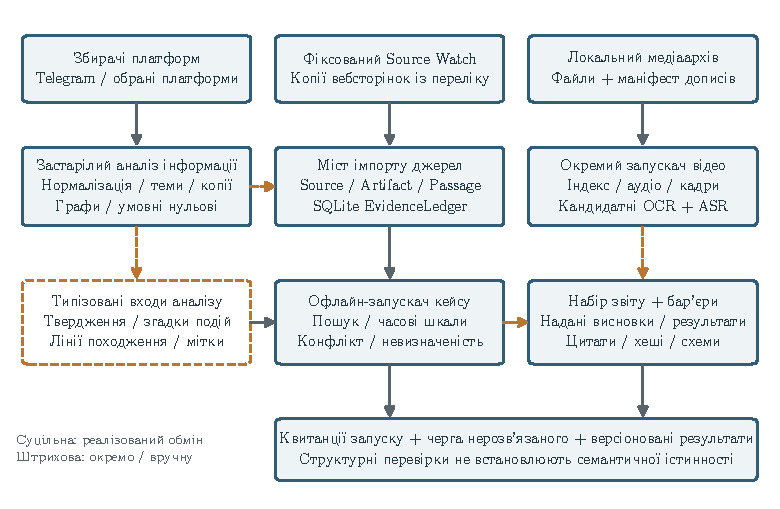
\includegraphics[width=\linewidth]{system_architecture.pdf}
\caption{Реалізовані компоненти Social та межі інтеграції на аудитованій ревізії. Суцільні стрілки позначають реалізований обмін; штрихові --- ручні або окремо запущені адаптери. Медійна й застаріла аналітична гілки виконувані, але загальний запускач інциденту оркеструє не всі з них.}
\label{fig:architecture}
\end{figure}

\begin{table}[!htbp]
\caption{Компоненти системи: реалізація й валідація є окремими вимірами. Шляхи вказано відносно кореня репозиторію; більшість аналітичних модулів розміщено в \code{src/analysis/}.}
\label{tab:components}\small
\begin{tabularx}{\linewidth}{@{}p{25mm}X p{25mm}@{}}\toprule
Компонент & Конкретна реалізація та роль & Свідчення готовності\\\midrule
Отримання даних & \code{src/tg_collect.py}, \code{src/tg_comments_collect.py}, \code{src/source_watch_collect.py}; окремі API- та вебзбирачі & Реалізовано; залежить від доступу, офлайн-тести\\
Підготовка знімків & \code{build_continuation.py}, \code{prep.py}; перевірене об'єднання й правила релевантності кейсу & Реалізовано; перевірки походження; семантична релевантність незалежно не валідована\\
Аналіз інформації & \code{analyze.py}, \code{coordination_lsh_audit.py}, \code{coordination_null_models.py} & Реалізовано; оцінено точний граф і обмежене повторне виконання\\
Облік доказів & \code{src/evidence_ledger.py}, \code{source_ingest_bridge.py}, \code{source_lineage.py} & Реалізовано; структурні тести й тести посилань\\
Оцінка доказів & \code{claim_verification.py}; BM25, евристики, агрегація & Пошук реалізовано; семантичні евристики експериментальні\\
Події та конфлікт & \code{event_reconstruction.py}, \code{conflict_analysis.py}; надані типізовані записи & Реалізовано впорядкування; фізичну істинність не оцінено\\
Локальні медіа & \code{src/media_pipeline.py}, \code{video_pipeline_runner.py}, \code{media_fingerprints.py} & Реалізовано; технічні квитанції; семантичні пороги не калібровані\\
Аналітика аудиторії & \code{audience_response.py}, \code{audience_aggregation.py} & Реалізовано контракти й агрегацію; мітки надані, точність не оцінено\\
Процес і звіти & \code{offline_case_runner.py}, \code{incident_orchestrator.py}, \code{report_generator.py}, \code{evaluation_harness.py} & Протестовано обмежену інтеграцію; наскрізне розслідування не валідоване\\\bottomrule
\end{tabularx}
\end{table}

Розрізнення в таблиці~\ref{tab:components} має операційне значення. Контрактні перевірки, вставлення в реєстр лише з додаванням і детерміновані процесори є повторно використовуваними механізмами. Переліки тверджень, обрані набори уривків, інтервали фізичних подій і еталонні рядки ASR в окремих збирачах є кураторськими дослідницькими входами. Скрипти досьє форматують результати; вони не перевіряють незалежно кожне емпіричне твердження, яке друкують. Схеми платформ можуть оголошувати платформу без наявного власного збирача. Жодну із цих категорій не слід зводити до твердження про готовність усього репозиторію до промислового використання.

\subsection{Зберігання та інтерфейси виконання}
Знімки JSON і JSONL забезпечують потокові записи й придатні для перегляду проміжні результати. CSV використовується для ребер графів, підсумків та окремих оцінювальних таблиць. SQLite зберігає зв'язані записи доказів. Сирі медіа й більші похідні зберігаються поза відстежуваними файлами коду, а маніфести пов'язують спостереження з байтами й похідним текстом. PDF і Markdown є формами подання, а не авторитетною заміною машинозчитуваних результатів.

Повторно використовуваний процес приймає \code{IncidentSpec}, явні типізовані входи, каталог результатів і ревізію Git виробника. Він фіксує поетапні квитанції та маніфест запуску. Викликач має надати справжню ревізію: запис рядка ревізії не доводить, що виконуваний код їй відповідав. Виконання обмежують бюджети, граничні часи, обмеження шляхів, обмежені розміри входів і явні стани \code{not_run}. Такий підхід віддає перевагу локальній придатності для перегляду й поступовому використанню на невеликій дослідницькій робочій станції, а не розподіленій агентній платформі, і залишає значну інтеграційну роботу на межі між збирачем і типізованим записом.

\section{Збір даних, нормалізація та походження}
\subsection{Отримання даних за джерелами}
Отримання даних Telegram використовує як автентифікований клієнтський доступ, так і публічні вебсторінки. Збирачі зберігають доступні ідентифікатори повідомлень, текст або підписи, час публікації, метадані каналів, інформацію про пересилання та лічильники на момент знімка. Збирач коментарів проходить доступні пов'язані обговорення, зберігає ідентифікатори гілок і відповідей та псевдонімізує ідентифікатори авторів. Інкрементне виконання й контрольні точки зменшують повторне отримання даних, але не встановлюють, що видалені, приватні, недоступні або не обрані матеріали було відновлено. Позначка повноти збирача стосується процедури посторінкового проходу й доступу на той момент, а не всіх можливих записів платформи.

\begin{table}[!htbp]
\caption{Фактична підтримка джерел. Реалізований доступ відрізняється від успішного й повного збору.}
\label{tab:sources}\small
\begin{tabularx}{\linewidth}{@{}p{24mm}p{45mm}X@{}}\toprule
Джерело & Реалізований доступ / дані & Основна межа\\\midrule
Telegram & Telethon/API і публічний веб; дописи, обрані обговорення, лічильники; окремий медіаархів & Цільова панель; обмеження автентифікації й доступу; ідентичність пов'язаного обговорення відрізняється від ідентичності допису каналу\\
Реакції Telegram & Нормалізація знімків MTProto; звичайні, користувацькі й платні реакції, якщо їх повернуто & Лише спостережений знімок; поточні лічильники не відновлюють минулу історію реакцій\\
YouTube & Скрипти \code{yt-dlp} для метаданих і коментарів інциденту; окремий збирач субтитрів & Ранжовані запити й обрані відео; ліміти коментарів, збої доступу та наявність субтитрів\\
TikTok & Публічний збір коментарів до окремих відео; вручну наданий набір URL & Обмеження платформи, обрані посилання; вичерпання посторінкового проходу не є повнотою генеральної сукупності\\
Instagram & Скрипт для інциденту на основі Instaloader і робота з кандидатними URL & Реалізований скрипт не встановлює успішного змістовного доступу\\
Офіційний веб і медіа & Фіксований дозволений перелік Source Watch; байти сторінок, метадані, виділений текст; допоміжні засоби архівування & Поточна доступність, фіксовані джерела; без вичерпного автономного пошуку\\
Facebook, Threads, X & Словник платформ / ручні або загальні URL-посилання & В аудитованому коді власного збирача не виявлено\\\bottomrule
\end{tabularx}
\end{table}

Обробка реакцій Telegram потребує окремого уточнення. MTProto надає типізовані результати реакцій і додаткові подробиці залежно від доступу \citep{telegram2026reactions}; Social має нормалізацію знімків і перевірку паритету на десяти коментарях. Історичний корпус коментарів не містить повного розподілу емодзі для всіх обраних гілок. Реакції на дописи й реакції на повідомлення в обговореннях не можна об'єднувати як той самий об'єкт. Відсутні дані, приховані дані, незібрані поля й виміряний нуль мають різне значення. Жоден поточний знімок не відновлює послідовність минулих голосів або кількість людей, які побачили коментар.

Source Watch фіксує статус HTTP, кінцевий URL, тип вмісту, обмежені байти, хеші та окремі метадані відповіді. Він відрізняє помилки від успішних змін сторінки й зберігає останню успішну базу порівняння під час збоїв. Отже, помилки TLS або HTTP описують невдале спостереження, а не відсутність офіційної заяви. Збережена помилка сертифіката не встановлює конкретної постійної причини в національній інфраструктурі сертифікатів. Отримання джерел неоднорідне: деякі старіші збирачі зберігають менш повний зв'язок між сирим тілом відповіді й нормалізованим результатом, ніж новіший вебміст.

\subsection{Нормалізація та ідентичність корпусу}
Застаріла попередня обробка вилучає окремі шаблонні фрагменти, нормалізує текст, застосовує прості мовні евристики й перевіряє правила релевантності для конкретного інциденту. Ці правила реалізовано, але вони не є незалежно валідованими багатомовними моделями релевантності. Фіксований зсув UTC для листопада в застарілому шляху обробки не є загальною системою часу з урахуванням переходів на літній час. Пізніша обробка продовження перевіряє маніфести завершених знімків і хеші, зберігає кілька спостережень на канонічне повідомлення та документує, яке спостереження дає обраний лічильник чи текст. Аналіз усе одно має вказувати точне обране поле й версію корпусу.

Публікаційний аудит виявив істотну помилку знаменника в раніших оповідних звітах. В історичному знімку з 23\,350 записів відсутні 459 сирих текстів і 49 лічильників переглядів; серед його 1\,408 релевантних записів обидва показники дорівнюють нулю. Придатні для аналізу схожості 1\,384 записи виключають 24 короткі релевантні тексти, а не 459 відсутніх. Окремий розширений знімок містить 23\,386 записів загалом і 1\,438 релевантних. Це різні файли з різними хешами, обраними каналами й результатами попередньої обробки. Чиста різниця не свідчить, що один корпус є лише доповненням іншого. Кожен наведений результат прив'язано до його фактичного вхідного хешу.

\subsection{Чотири різні гарантії походження}
\emph{Технічне походження} фіксує URI джерела, часові позначки збору й публікації, ідентичність артефакта, хеші, версії перетворень і локатори. \emph{Інформаційне походження} показує, як твердження виводиться з попереднього джерела. \emph{Незалежність доказів} ставить питання, чи додають формально різні матеріали незалежне спостереження. \emph{Семантична обґрунтованість} ставить питання, чи справді цитований уривок обґрунтовує висновок. W3C PROV розрізняє сутності, дії, агентів, виведення й атрибуцію \citep{lebo2013provo,moreau2013provdm}; Social використовує споріднені ідеї через типізовані записи, а не через продемонстрований експорт RDF, сумісний зі стандартом.

Хеш захищає побайтове порівняння, а не автентичність чи істинність. Реєстр перевіряє синтаксис хешу; фактичні перевірки байтів виконуються в компонентах імпорту. Його загальний локатор уривка необов'язковий, тому точні зміщення не є інваріантом усієї базової ревізії. Міст Source Watch перевіряє байти зібраного тіла відповіді, але довіряє виділеному тексту, наданому збирачем; він незалежно не перезапускає й семантично не валідує виділення. Тригери SQLite лише з додаванням перешкоджають звичайним оновленням і видаленням через цей інтерфейс бази даних, але не роблять локальну базу захищеною від підробки її власником. Ці розрізнення необхідні для обґрунтованого криміналістичного використання \citep{berkeleyProtocol2022}.

\section{Аналіз інформаційних хвиль}
\subsection{Часова й наративна обробка}
Social формує підсумки за часом публікації, інтервали активності, графи видимих пересилань і лексичні наративні мітки. Багатоміткова кодова книга охоплює теми заручників і утримання, смерті й катувань, «табору ТЦК», приховування та офіційної реакції. Це тематичні виявлення, а не перевірені факти чи переконання аудиторії. Пізніший \code{narrative_v3.py} додає структуровані розрізнення й правила утримання від рішення, але його модульні приклади не становлять нового незалежно встановленого бенчмарка точності. На збереженому порівнянні 40 дописів із мітками Claude застаріла точність/повнота для N1 становить 0,20/0,25, для N2 --- 0,18/0,40; N4 не має істинно позитивних збігів. Ці порівняння показують розбіжності, а самі ШІ-мітки також лишаються невизначеними.

Тема, наратив, твердження й позиція мають різні ролі. Тема вказує предмет обговорення; наратив організовує інтерпретаційну оповідь; твердження є обмеженим судженням; позиція описує ставлення тексту до цільового судження. Наявність ключового слова не може встановити прихований мотив чи політичну належність людини. Тому це оцінювання використовує кількість наративів лише як лексичні показники й не тлумачить їх як калібровану поширеність. Українські бенчмарки емоцій ілюструють потребу в оцінюванні для конкретної мови \citep{dementieva2025emobench}, а не автоматичну обґрунтованість наданих Social міток аудиторії.

\begin{table}[!htbp]
\caption{Алгоритми та продемонстрований обсяг їх вимірювання.}
\label{tab:algorithms}\small
\begin{tabularx}{\linewidth}{@{}p{31mm}X X@{}}\toprule
Техніка & Реалізація / завдання & Межа перевірки\\\midrule
Regex і нормалізація & \code{prep.py}, \code{narratives.py}, \code{narrative_v3.py}; релевантність і теми & Правила й регресії; обмежене порівняння з ШІ-мітками\\
MinHash/LSH, точний Jaccard & \code{analyze.py}, \code{coordination_lsh_audit.py}; кандидатний і точний граф копій & Вичерпне повторне обчислення графа й повноти на скінченному корпусі\\
Умовна рандомізація & \code{coordination_null_models.py}; відхилення шаблонів і часу & Підсумки нульових моделей на фіксованих входах і відтворення префікса із зерном\\
Статистика графів & \code{telegram_network_dynamics.py}; видимі пересилання й часові інтервали & Звірка степенів, обсягів та інтервалів; без причинного висновку про мережу\\
BM25 і правила відношень & \code{claim_verification.py}; кандидати-уривки й обмежені оцінки & Контракти пошуку й локаторів; продемонстровані семантичні збої правила\\
Часові обмеження & \code{event_reconstruction.py}; надані згадки подій & Порядок інтервалів і заборони зв'язування; без оцінки істинності фізичних подій\\
Перцептивні хеші, ASR/OCR & \code{media_fingerprints.py}, \code{video_text_extract.py} & Технічні квитанції й порівняння тексту з наданим еталоном; некалібровані візуальні пороги\\\bottomrule
\end{tabularx}
\end{table}

\subsection{Повторення тексту як обмежене завдання пошуку}
Для нормалізованих текстів застаріла реалізація будує множини п'ятисимвольних шинглів, використовує 128 перестановок MinHash і пошук кандидатів LSH, а потім обчислює точну подібність Jaccard для кандидатів. Для множин шинглів $A,B$
\begin{equation}\label{eq:jaccard}
J(A,B)=\frac{|A\cap B|}{|A\cup B|}.
\end{equation}
MinHash є ефективним наближенням подібності \citep{Broder1997}; LSH може пропускати пари, що відповідають умові. Вичерпний аудит Social натомість обчислює розріджені цілочислові перетини на всьому придатному корпусі повних текстів і виключає пари в межах одного каналу. Реалізаційний контроль запобігає переповненню довгих перетинів. Повнота 367/369 в аудиті обумовлена цим точним графом шинглів і визначенням придатності. Це не повнота виявлення семантичних перефразувань і не точність виявлення інформаційних операцій. Відтворення скінченного графа є корисним алгоритмічним результатом саме тому, що його знаменник явно визначений.

\subsection{Поведінкові сигнали та умовні нульові моделі}
Копіювання, спільна поява й синхронізовані дії є усталеними сигналами аналізу координації \citep{Pacheco2021,Nizzoli2021,Magelinski2022}. Social перевіряє обрані статистики шаблонів коментарів і часу копіювання дописів за умовної рандомізації. Моделі коментарів зберігають задані страти день/активність/письмо або автор/день. Моделі часу циклічно зсувають зайняті слоти публікації в межах локальних для каналу блоків по 24 або дві години. Один рандомізований час на вузол використовується на всіх інцидентних ребрах графа, що зберігає залежність через спільні вузли, а не трактує ребра як незалежні випробування.

Для статистики верхнього хвоста $T$, $B$ випадкових вибірок і спостереженого $T_{obs}$ реалізація використовує
\begin{equation}\label{eq:permutation}
\widehat p=\frac{1+\sum_{b=1}^{B}\mathbf{1}[T_b\geq T_{obs}]}{B+1},
\end{equation}
після чого застосовано поправку Голма для визначеної сім'ї з 16 тестів \citep{Phipson2010,Holm1979}. Центральний діапазон рандомізації не є довірчим інтервалом для генеральної сукупності. Це розвідувальні відхилення від явних моделей обмінюваності. Спільні новинні шоки, синдикований текст, легітимне адміністрування каналів і органічне копіювання лишаються можливими поясненнями. Статистична синхронізація не встановлює неавтентичної поведінки, операційної координації, організаційного контролю чи державної атрибуції.

\subsection{Класифікація каналів та інтеграція аудиторії}
У деяких графах лишаються застарілі групи каналів. Новіший \code{channel_evidence.py} натомість фіксує інфраструктурні маркери й окремі осі атрибуції, а за замовчуванням вважає походження й орієнтацію невідомими, а операційну атрибуцію неперевіреною. Російська мова, домен чи посилання на платформу не є доказом державного контролю. Сценарний аналіз може показати, як припущена належність до групи змінює підрахунки, але не може калібрувати невідому власність за цими маркерами.

Контракти реакції аудиторії підтримують коментарі, зв'язки відповідей, знімки реакцій, цілі, надані семантичні мітки й агрегати. Досліджений адаптер нормалізує мітки, а не виводить незалежно теми, емоції чи позиції з кожного коментаря. Його результати зберігають \code{semantic_quality_status=not_evaluated}. Підсумки зі зважуванням за коментарями, авторами, гілками й каналами мають різні цільові величини; жодне зважування не робить цілеспрямовано спостережені обговорення репрезентативними для населення країни. Тому стаття описує інфраструктуру й охоплення аудиторії без вигаданих рейтингів локальних класифікаторів чи поширеності емоцій.

\section{Облік доказів та обмежена перевірка}
\label{sec:evidence}

Доказовий шар розділяє твердження джерела, його архівоване подання та подальшу оцінку. Конкретною реалізацією є клас Python \code{EvidenceLedger}, який зберігає версіоновані записи JSON у SQLite. Назви записів у таблиці~\ref{tab:evidence} позначають дискримінатори словників, а не сім відповідних класів Python. Функції аналізу окремо обмінюються JSON-сумісними документами, валідованими за схемами. Їхні зв'язки походження концептуально споріднені з PROV, але експорт RDF чи відповідність PROV-O не продемонстровано \citep{moreau2013provdm,lebo2013provo}.

\begin{table}[!htbp]
\centering
\small
\caption{Конкретні види записів реєстру та забезпечувані межі. Посилальна цілісність встановлює простежуваність, але не встановлює доказового логічного випливання.}
\label{tab:evidence}
\begin{tabularx}{\linewidth}{@{}lXX@{}}
\toprule
Вид запису & Збережений вміст і зв'язки & Основне структурне обмеження \\
\midrule
Source & URI, назва, видавець, час публікації & Ідентифікатор і обов'язкові метадані \\
Artifact & Зв'язок із джерелом, шлях, дайджест, час збору & Наявне джерело; синтаксис SHA-256 \\
Passage & Зв'язок з артефактом, текст, локатор & Наявний артефакт; непорожній текст \\
Claim & Твердження, тип, зв'язки з джерелами й доказами & Атрибутоване джерело або докази висновку \\
ClaimMention & Зв'язки із твердженням та уривком & Оприлюднене твердження й уривок із того самого джерела \\
EvidenceAssessment & Твердження, статус, докази, обґрунтування & Дійсні посилання й ланцюг заміщення \\
VerificationResult & Обсяг, гранична дата, статус, сторони доказів & Узгоджені зі статусом посилання на докази \\
\bottomrule
\end{tabularx}
\end{table}

Реєстр відхиляє оновлення й видалення через тригери SQLite. Повторне вставлення ідентичного запису ідемпотентне; повторне використання ідентифікатора з іншим вмістом завершується помилкою. Оцінки й результати перевірки можуть заміщувати попередні записи, не замінюючи їх, причому заміщення має стосуватися того самого твердження й не може розгалужуватися. Дайджест артефакта перевіряється за форматом, а не обчислюється реєстром заново з архівованого файлу. Локатор уривка може містити довільний JSON; перевірка точного текстового фрагмента належить окремому конструктору оцінки. Ці розрізнення показано на рисунку~\ref{fig:provenance}.

\begin{figure}[!htbp]
\centering
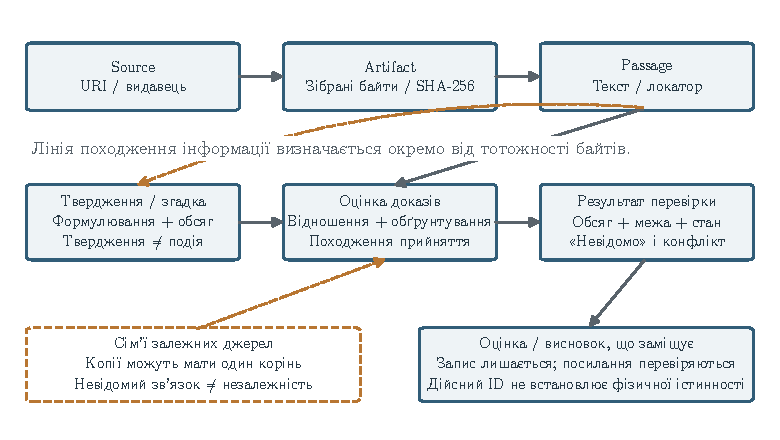
\includegraphics[width=\linewidth]{evidence_provenance.pdf}
\caption{Зв'язки доказів і походження. Твердження джерел, байти артефактів, виділені уривки й аналітичні судження лишаються окремими. Зафіксована лінія походження й дійсні локатори підтримують перевірку, але не гарантують істинності чи незалежності джерел.}
\label{fig:provenance}
\end{figure}

Локальний пошук використовує BM25 на наданих уривках, шукає в напрямах твердження та контрдоказів і дотримується граничного часу збору й бюджету запитів. Результати лишаються неоціненими кандидатами. Конструктор оцінки перевіряє, що цитований фрагмент у кодових точках Unicode дорівнює підрядку уривка, валідує обсяг і числові обмеження та фіксує походження прийняття. Прийняті оцінки потребують мітки людського рішення або мітки валідованого правила з ідентифікатором правила. Це структурна вимога: конструктор не звертається до незалежно валідованого реєстру правил. Спеціалізований збирач тверджень надає другу мітку програмно.

Спільний словник перевірки містить сім станів: \code{unverified}, \code{supported_within_scope}, \code{refuted_within_scope}, \code{conflicting_evidence}, \code{insufficient_evidence}, \code{not_verifiable} і \code{superseded}. Він виключає оцінки, що є лише кандидатами, не відповідають часу чи обсягу або неналежно процитовані. Пороги вердикту рахують оголошені ідентифікатори ліній походження; окремі поля рахують корені, явно позначені як незалежно підтверджені. Ці величини не можна змішувати. Обсяг фізичного факту додатково вимагає прийнятої прямої фізичної доказової основи, перш ніж підтримка чи спростування можуть бути чинними. Тому заперечення установ може лишатися зафіксованим як офіційна позиція, тоді як доказів фізичного твердження бракує. Цей запобіжник залежить від наданого типу обсягу; він незалежно не класифікує епістемічний обсяг твердження.

Кураторський пакет кейсу містить 25 тверджень, 25 обраних уривків і 36 прийнятих оцінок за правилом. Його поточні результати за схемою~2.3 --- 19 підтриманих, нуль спростованих і шість із недостатніми доказами. Це вихідні дані програми, а не вимірювання точності. Раніший пакет за схемою~2.0 давав 21 підтриманий і чотири спростовані результати з 31 оцінки, вставляючи визначені уривки й очікувані відношення в побудову оцінок. Поточний код оцінює лише знайдених кандидатів і усуває це пряме вставлення, але твердження, запити, уривки, обсяги й мітки ліній походження лишаються кураторськими. Загальний офлайн-запускач обмеженіший: він шукає кандидатів і не створює прийнятих оцінок.

Два спеціально сконструйовані випробування показують семантичні збої базового зіставлювача; пізнішу ревізію оцінено в розділі~\ref{sec:rule-v2}. Уривок про 26 дерев приймається як підтримка твердження про 26 військових у будівлі, а речення із запереченням прибуття поліції --- як підтримка прибуття. Обидва отримують фіксовану впевненість гілки 0,92. Збережений артефакт кейсу також приймає уривки про травми й самостійне пересування як підтримку твердження про чотирьох осіб, які самовільно залишили частину. Збіг чисел може задовольнити правило підтримки без збігу присудка, а лексичне перекриття може пропустити звичайне заперечення. Крім того, висновок використовує весь уривок, тоді як збережена цитата може бути коротшим знайденим фрагментом. Тому точне цитування не гарантує, що цитата логічно обґрунтовує призначене відношення.

Жоден незалежний локальний еталонний набір не встановлює точності логічного випливання й не калібрує ці значення впевненості. Випробування демонструють збої, а не оцінюють їх поширеність. FEVER і AVeriTeC обґрунтовують спільне оцінювання достатності доказів і правильності вердикту \citep{thorne2018fever,schlichtkrull2023averitec,schlichtkrull2024averitec}, але не замінюють оцінювання цієї системи на незалежно встановлених твердженнях. InFact є зовнішнім поетапним орієнтиром \citep{rothermel2024infact}, а не виміряною тут базовою лінією.

\section{Згадки подій і два часові шари}
\label{sec:events}

Реконструкція подій приймає вже типізовані згадки, що містять присудок, ідентифікатори учасників та об'єктів, місце, посилання на докази й часові метадані. Вона не виділяє події автономно зі звітів, дописів чи відео. Ця межа відрізняє її від контрольованого виділення на основі фрагментів, де передбачені тригери й аргументи оцінюються за анотованим текстом \citep{wadden2019dygiepp}. Реалізований внесок --- консервативне впорядкування наданих тверджень.

Згадки комунікацій використовують час публікації; фізичні згадки потрапляють на свою часову шкалу лише за наданих найранішої й найпізнішої меж часу події. Відсутній або частково обмежений фізичний час зберігається без заміни часом публікації. Два шари показано на рисунку~\ref{fig:dual}. Попарні порівняння інтервалів дають відношення «раніше», «пізніше», «перекриття» або «невідомо», а кожне часове ребро явно позначене як непричинне. Упорядкування повідомлень не може встановити, що одна фізична дія спричинила іншу.

\begin{figure}[!htbp]
\centering
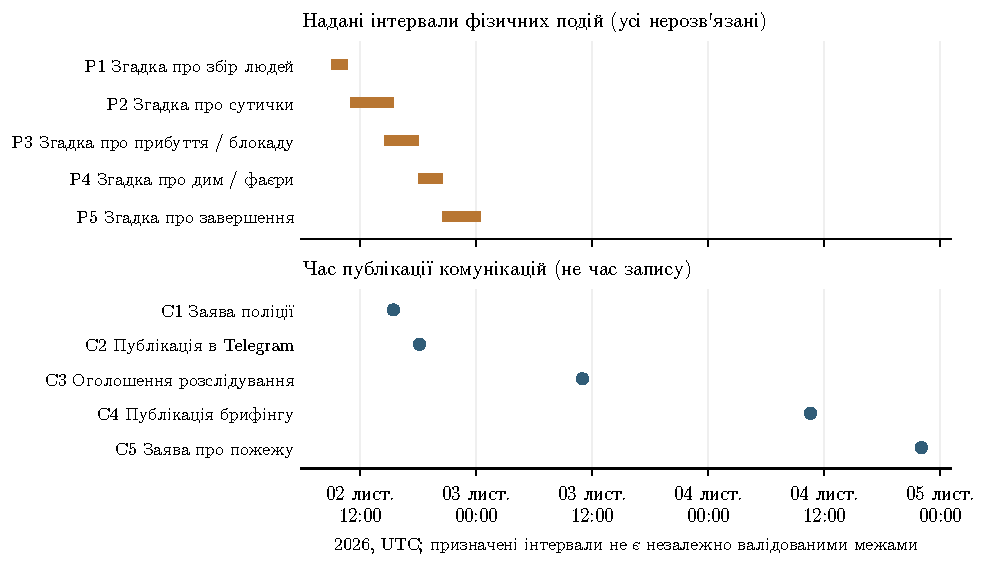
\includegraphics[width=\linewidth]{dual_timeline.pdf}
\caption{Окремі часові шкали комунікацій і фізичних подій. Час публікації визначає положення комунікацій; надані аналітиком інтервали --- положення повідомлених фізичних епізодів. Перекриття меж і нерозв'язані згадки лишаються видимими, а часовий порядок не має причинного тлумачення.}
\label{fig:dual}
\end{figure}

Точний збіг нормалізованого присудка, ідентифікаторів учасників і об'єктів та місця може створити придатний для перегляду зв'язок «можливо та сама подія» за умови часової сумісності й наданих заборон зв'язування. Функція ніколи не об'єднує згадки. Така стриманість важлива, бо подібні описи можуть стосуватися різних випадків подій; цю складність підкреслює ECB+ \citep{cybulska2014ecbplus}. Заборони зв'язування зберігають розрізнення, задані аналітиком; вони не є незалежно виявленими судженнями про тотожність.

Кураторська хронологія містить п'ять фізичних і п'ять комунікаційних згадок. Усі десять лишаються нерозв'язаними, зв'язків «можливо та сама подія» немає. Учасники, інтервали, позиції сторін і якісні рівні доказів задані в буквальному вхідному списку збирача. Ці рівні описують заявлену доказову основу, а не калібровану впевненість чи перевірене фізичне відбуття. Отже, артефакт демонструє відтворюване часове впорядкування та явну невизначеність; його підрахунки не вимірюють повноту виявлення подій чи точність реконструкції.

\section{Обробка мультимодальних доказів}
\subsection{Технічне отримання та похідні}
Мультимодальна обробка починається з ідентичності локального файлу та технічної читабельності, а не з інтерпретації сцени. \code{media_pipeline.py} обчислює SHA-256 потоково, досліджує медіа й може виконувати суворе декодування всього файлу через FFmpeg. Окремий запускач відео адаптує маніфести завантаженого архіву, валідує локальні файли, створює похідні аудіо та вибіркові кадри й за потреби викликає OCR і ASR. Повторне використання кешу залежить від вмісту, параметрів, моделі й конфігурації та відбитків коду. Атомарний запис і перевірки stat зменшують випадкове повторне використання неповних результатів. Це реалізовані інженерні засоби контролю, а не твердження про криміналістичну сертифікацію автентичності.

\begin{figure}[!htbp]
\centering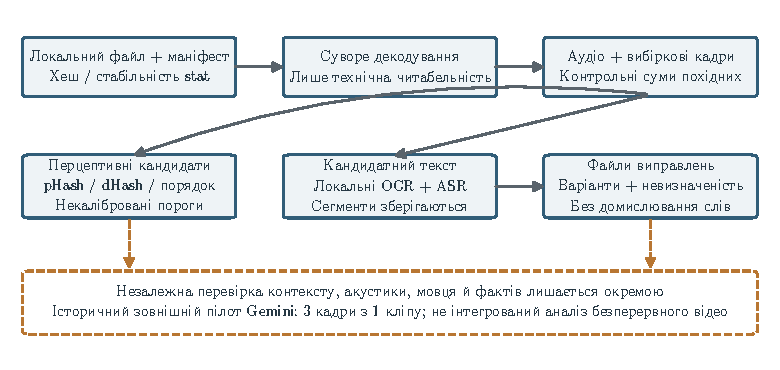
\includegraphics[width=\linewidth]{multimodal_pipeline.pdf}
\caption{Реалізований локальний мультимодальний конвеєр. Технічна обробка створює придатні для перегляду кандидатні спостереження. Незалежна акустична, контекстуальна, особова перевірка й перевірка подій є окремими завданнями; історичний зовнішній пілот Gemini на трьох ключових кадрах не входить до цього автоматизованого запускача.}
\label{fig:media}
\end{figure}

Порівняння вибіркових кадрів поєднує 63-бітний низькочастотний перцептивний хеш DCT і 64-бітний горизонтальний різницевий хеш. Воно оцінює повні кадри, кадри з обрізаною рамкою та центральні кадри, зокрема горизонтальні дзеркальні варіанти, і виключає малоінформативні кадри. Правило кандидатів за замовчуванням використовує межі Геммінга 10 і 12, щонайменше 0,6 часово узгодженого покриття коротшого проаналізованого вікна, три різні збіжні кадри й хеші та двосекундний проміжок. Зміщення найближчих кадрів і їхнє медіанне відхилення описують відносне вирівнювання послідовності. Ці розвідувальні пороги не є каліброваними ймовірностями збігу. Подібні накладення, статичні сцени та ефекти добору можуть давати хибнопозитивні результати; рідкісна вибірка, монтаж і кадрування --- хибнонегативні. Ані збіг, ані його відсутність не встановлюють місце запису, тотожність події, напрям копіювання чи автентичність.

\subsection{Кандидатне мовлення й текст}
Необов'язковий текстовий шлях використовує Tesseract OCR і faster-whisper ASR. OCR видає рамки слів і часові позначки, пов'язані з кадрами; ASR --- сегменти тексту з часом. Усталена архітектура OCR Tesseract і багатомовне навчання Whisper дають корисну основу для виділення тексту \citep{smith2007tesseract,radford2023whisper}. Їхні опубліковані результати не кількісно визначають роботу конкретних конвертованих моделей на українських, російських, змішаних за мовою чи зашумлених записах Social. Налаштування виконання й декодування faster-whisper також потребують явного версіонування \citep{systran2026faster}.

Історичні масові квитанції вказують CPU/int8 \code{Systran/faster-whisper-small}, ревізію \code{536b0662742c02347bc0e980a01041f333bce120} і faster-whisper 1.1.0. Обраний другий прохід по семи активах використовував \code{mobiuslabsgmbh/faster-whisper-large-v3-turbo}, ревізію \code{0a363e9161cbc7ed1431c9597a8ceaf0c4f78fcf}. Цей добір не є контрольованим порівнянням моделей на всьому корпусі. Початковий та альтернативний тексти зберігаються як супровідні файли виправлень; десять лексичних кандидатів у цьому перегляді лишаються \code{quote_safe=false}. Правдоподібного контекстуального формулювання недостатньо, щоб мовчки заповнювати нерозбірливе мовлення.

Безпека цитування має кілька окремих вимог: текст має відповідати аудіо, ім'я мовця має бути обґрунтованим, цитата має зберігати контекст, а фактичні твердження всередині цитати потребують власної оцінки доказів. Бенчмарк із 18 кліпів зберігає десять позначок \code{quote_safe=true}, але ідентифікатор ШІ-виконавця поряд із полем «людське акустичне прослуховування» незалежно не доводить участі людини-слухача. Наведено арифметику помилок відносно наданого еталона й зафіксовані позначки, а не незалежно перевірену безпеку цитування. Неочікувано вища помилка в номінальній страті чистого мовлення не може встановити загальний ефект шуму: кліпи, термінологія й побудова еталонів різняться, а кліпів у страті лише кілька.

\subsection{Здійсненність зовнішньої моделі та інтеграція}
Історична квитанція описує пілот користувацького Agy Gemini 3.8 Flash на трьох нерухомих кадрах з одного кліпу тривалістю 15,278 секунди. Спробу обробки повного відео заблоковано, а запуск на ключових кадрах повернув кандидатні візуальні спостереження. Це свідчення здійсненності виклику зовнішнього інструмента без валідації безперервного відео, аудіо, геолокації, особи, істинності чи точності. Поточний запускач Python не містить автоматичного виклику Gemini/Agy. Наведені кількості токенів не є виміряною грошовою вартістю, а результати іншої моделі не є незалежним підтвердженням сцени.

\section{Автономний процес і надійність}
\subsection{Що саме автоматизує контролер}
Оркестратор інциденту приймає типізовану специфікацію інциденту, фіксовані входи аудиту Source Watch і бюджети ресурсів. У режимі виконання його реєстр у коді може викликати наявний вебзбирач із дозволеного переліку. Початкові URL не розширюють автоматично цей реєстр або перелік дозволених доменів. Нові маніфести збору можуть проходити через міст імпорту до локального для запуску реєстру доказів. Після цього можуть оброблятися необов'язкові типізовані офлайн-входи. Планування без виконання, виконання збору й локальний аналіз є явними незалежними опціями.

Офлайн-запускач викликає лінії походження, пошук, типізоване впорядкування часової шкали, інформаційні підсумки, надані входи конфлікту, сценарії невизначеності та перевірки звіту, якщо є сумісні входи. Відсутні входи він фіксує як заблоковані або не запущені, а не вигадує їх. Пошук не викликає евристик прийняття кураторського збирача тверджень. Формування звіту очікує окремо наданий набір із висновками, записами доказів і результатами перевірки. Тому успішне виконання контролера не свідчить, що сирі джерела автономно перетворено на перевірені висновки. Вирішальну межу показано на рисунку~\ref{fig:workflow}.

\begin{figure}[!htbp]
\centering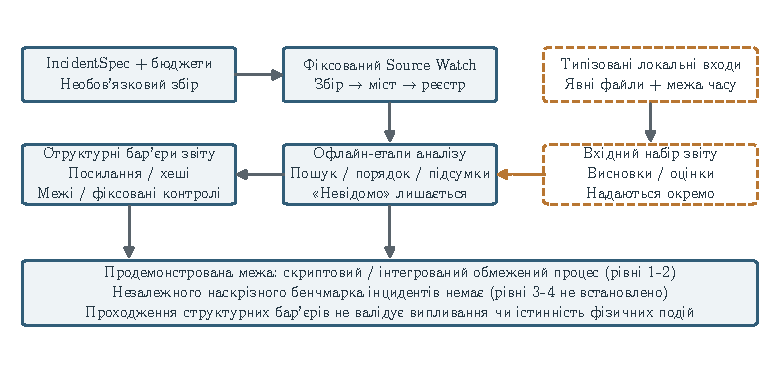
\includegraphics[width=\linewidth]{analysis_workflow.pdf}
\caption{Обмежений процес і межі автоматизації. Типізовані входи, кураторські судження й окремо запущений аналіз медіа надходять через явні інтерфейси. Структурні бар'єри можуть відхилити недійсні посилання, але не можуть перетворити кандидатний уривок на семантично обґрунтований висновок. Твердження про наскрізне розслідування лишається невалідованим.}
\label{fig:workflow}
\end{figure}

\subsection{Явна описова шкала автономності}
У цій статті рівень~0 означає ручну роботу; рівень~1 --- скриптову обробку наданих входів; рівень~2 --- інтегрований автоматизований аналітичний процес; рівень~3 --- автономний пошук і оцінку з урахуванням доказів у межах незалежно валідованих завдань; рівень~4 --- незалежно валідований наскрізний аналіз інцидентів із початково невідомими результатами. Це авторська описова шкала, а не стандарт спільноти чи порядкова міра точності.

Більшість збирачів, локальне індексування й кураторські збирачі працюють на рівні~1. Типізований офлайн-запускач і обмежений оркестратор демонструють інтеграцію рівня~2. Їхні семантичні входи й висновки лишаються обмеженими наданими даними та невиміряною якістю висновування. Окремо виконаний евристичний збирач тверджень не підносить усю систему до рівня~3; жоден поточний результат не демонструє рівень~4. Людські або зовнішньо валідовані еталонні набори потрібні під час розробки й оцінювання, але це не означає, що людина має розмічати кожен майбутній запис під час експлуатації. Натомість непідтримувані завдання мають лишатися невідомими або поза межами валідованої робочої області.

\subsection{Контрольні бар'єри надійності та невизначеність}
Оцінювальний каркас перевіряє форму схем, посилання, граничні часи, залежності джерел, хеші артефактів звіту й зафіксовані синтетичні сценарії. Семантичне оцінювання він явно позначає як невиконане. Зокрема, 783 пройдені тести не можуть означати 100\% фактичної точності. Структурне походження прийняття, як-от \code{validated_rule}, не встановлює, що правило було незалежно валідоване. Фіксовані значення евристичної впевненості не є каліброваними ймовірностями.

Сценарії невизначеності показують залежність від спірних міток, невідомих груп каналів, припущень про вилучення й обмеження та сконцентрованих спостережень. Їхні інтервали є сценарними межами, обумовленими наданими записами, а не вибірковими довірчими інтервалами для суспільної думки. Інкрементний запуск і порівняння звітів можуть виявляти зачеплені результати та змінені рішення, але не гарантують істинності переглянутого змістового висновку. Інженерним пріоритетом є прозорий збій і придатність для перегляду, що узгоджується з практиками відтворюваних досліджень \citep{sandve2013reproducible,wilson2017practices}; семантична надійність лишається окремим емпіричним завданням.

\section{Оцінювання}
\label{sec:evaluation}

Оцінювання розділяє обчислювальну відтворюваність, поведінку детермінованих контрактів, описові вимірювання корпусу та семантичну правильність. Ці категорії мають різні еталони. Побайтово ідентичне повторне виконання встановлює повторюваність перетворення; негативний контроль --- відхилення заданого недійсного входу; жодне з них не встановлює істинності реконструйованої події. У таблиці~\ref{tab:evaluation} наведено всі десять системних експериментів із категорією доказів і межами, що лишаються. Машинозчитувані значення, хеші джерел, знаменники, середовище й команди супроводжують статтю у файлі \texttt{audited\_evaluation\_metrics.json}; журнали виконання зберігаються окремо. Для цих перевірок не знадобилося свіжого збору чи виконання моделей.

\begin{table}[!htbp]
\centering
\small
\caption{Матриця оцінювання системи. «Оцінено» означає вказане обмежене вимірювання, а не незалежну семантичну валідацію. Історичні квитанції відрізняються від свіжих перевірок.}
\label{tab:evaluation}
\begin{tabularx}{\textwidth}{@{}p{0.07\textwidth}p{0.19\textwidth}XX@{}}
\toprule
ID & Експеримент & Докази й спостережений результат & Межа оцінювання \\
\midrule
E1 & Відтворюваність & Свіжі перевірки хешів, повторне обчислення точного графа, арифметика збережених вибірок і чотири префікси по 25 вибірок збігаються. & Без свіжого повторного збору; повна генерація 9\,999 вибірок --- історична квитанція. \\
E2 & Збір даних & Збережені історичні й розширені підрахунки та пропуски незалежно перераховано. & Опис цілісності й охоплення; повнота платформ і повнота релевантності невідомі. \\
E3 & Виявлення дублікатів & Точний прохід: 369 пар, що відповідають умові; застарілі кандидати зберегли 367; два пропуски, нуль зайвих. & Умовна повнота кандидатів на скінченному корпусі; семантичного еталона дублікатів немає. \\
E4 & Виявлення координації & Збережена сім'я з 16 тестів: сире $p=0{,}0001$, $p$ за Голмом $=0{,}0016$; обмежені префікси відтворюються. & Умовні розвідувальні нульові моделі; специфічність щодо органічних подій і атрибуція не виміряні. \\
E5 & Пошук доказів & Пошук по зібраному корпусу та контролі посилань перевірено офлайн-тестами. & Кураторські відомі входи; сліпого бенчмарка пошуку у відкритому вебі немає. \\
E6 & Перевірка тверджень & Контрактні контролі утримання від рішення, конфлікту, граничного часу й ліній походження пройдено. & Незалежної оцінки семантичної точності чи випливання немає; авторський стрес-тест пізнішої ревізії правила наведено в розділі~\ref{sec:rule-v2}. \\
E7 & Реконструкція подій & Перевірено типізоване впорядкування подій і синтетичні інваріанти часової шкали та посилань. & Без автономного виявлення подій із сирих даних і незалежно встановленої оцінки хронології. \\
E8 & Відео/ASR & Історична арифметика відносно наданого еталона: 185 помилок на 415 слів, micro-WER 44,58\%. & Обрані кліпи; незалежне походження еталонного прослуховування не встановлено. \\
E9 & Наскрізний процес & Два чисті повтори лише з пошуком лишаються частковими й неперевіреними; негативний контроль із висячою подією не проходить. & Два кандидати, без прийнятої підтримки, без згенерованого звіту; це не сліпе оцінювання інциденту. \\
E10 & Час і ресурси & Свіжий офлайн-набір: 7,84\,с, максимум RSS 328\,320\,КіБ; виміряно й обмежений аналітичний аудит. & Часткові локальні навантаження; без поточного бенчмарка GPU, вартості API чи пропускної здатності повного запуску. \\
\bottomrule
\end{tabularx}
\end{table}

Свіжий повний набір тестів репозиторію на зафіксованій базовій ревізії дав 783 пройдені тести й 16 пройдених підтестів без збоїв на робочій станції, яка зберігає приватні корпуси. Pytest зафіксував 7,41\,с; зовнішнє вимірювання ресурсів --- 7,84\,с реального часу й максимум резидентної пам'яті 328\,320\,КіБ з успішним завершенням. Інтерпретатором був Python 3.13.14 віртуального середовища репозиторію на Linux/x86-64. Ці підрахунки описують регресійне покриття, а не знаменник точності. Також пройдено шість зафіксованих синтетичних контролів: відомий мікрокейс, розгалуження копій із одного кореня, суперечливі свідчення, граничні часи виправлень, неповні докази й повторно використане відео. Їхні очікувані стани відомі за побудовою. Вони корисні як бар'єри випуску, але не є сліпими спостереженнями істинності інцидентів.

Для обліку збору пряме читання файлів звірило 23\,350 історичних публікацій із 1\,408 обраними релевантними записами та 1\,384 текстами, придатними для аналізу схожості. Історичні 459 відсутніх сирих текстів і 49 відсутніх лічильників переглядів належать до всіх публікацій; у релевантній підмножині жоден із цих показників не відсутній. Решта 24 релевантні тексти коротші за поріг придатності у 80 символів. Розширений знімок містить 23\,386 публікацій і 1\,438 релевантних записів. Ці версії є окремими рамками аналізу. Точний граф і умовні часові тести використовують історичну рамку; приписування цього графа розширеній рамці в документі ліній походження відхилено за його зафіксованими вхідними хешами. Такі перевірки стосуються цілісності знаменників, не встановлюючи репрезентативності вибірки~\cite{Olteanu2019,VicentePaula2023}.

Експеримент із дублікатами заново обчислив весь придатний точний граф за визначенням п'ятисимвольних шинглів із робочого коду та 64-бітною арифметикою перетинів. За порогів Jaccard 0,60, 0,75 і 0,90 точні міжканальні підсумки становили 369, 288 і 213; застарілий пошук зберіг 367, 288 і 213. Отже, повнота кандидатів за порогу 0,60 дорівнює $367/369=99{,}45799458\%$ за умови 1\,384 придатних історичних текстів. Вісімнадцять пар у межах одного каналу виключено визначенням графа. Обидва пропущені міжканальні ребра мають лаг понад 30 хвилин, тому спостережені короткі лаги лишаються 134 у межах десяти хвилин і 198 у межах тридцяти, кожен із них тепер поділено на 369. На рисунку~\ref{fig:copy} показано це розрізнення між пошуком кандидатів і точним вимірюванням. Скетчинг шинглів забезпечує механізм пошуку, а не семантичну тотожність чи залежність джерел~\cite{Broder1997}.

\begin{figure}[!htbp]
\centering
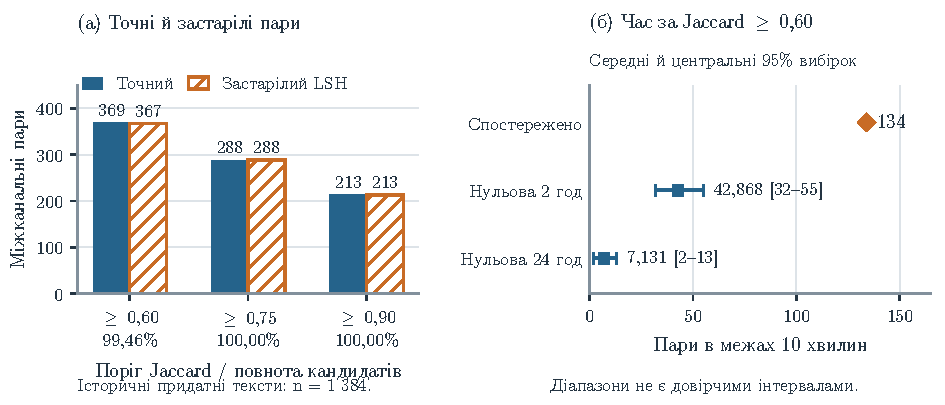
\includegraphics[width=\textwidth]{information_analysis.pdf}
\caption{Пошук схожості на скінченному корпусі та умовний час копіювання. Ліворуч: точні й збережені застарілим методом пари з повнотою для кожного порога серед 1\,384 придатних історичних текстів. Праворуч: 134 спостережені пари з Jaccard $\geq 0{,}60$ у межах десяти хвилин порівняно із середніми двох збережених умовних нульових моделей. Вуса показують центральні 95\% із 9\,999 рандомізованих вибірок, а не довірчі інтервали. Усі часові підрахунки використовують фіксований граф із 369 ребер. Джерела й хеші збережено в \texttt{data/figure\_data/information\_analysis.json}.}
\label{fig:copy}
\end{figure}

Для координації кожну збережену вибірку перечитано, а всі шістнадцять підсумкових рядків обчислено заново, зокрема середні, квантилі, верхні включні хвости й поправку на множинність. За 9\,999 вибірок усі зафіксовані кількості перевищень дорівнюють нулю; значення Монте-Карло з додаванням одиниці становить $(0+1)/(9999+1)=0{,}0001$, а поправка Голма для оголошеної сім'ї дає 0,0016~\cite{Phipson2010,Holm1979}. Свіже повторне виконання відтворило перші 25 вибірок кожної з чотирьох моделей із зерном 20261106. Цей аудит не генерував заново всі вибірки. Часові перестановки призначають кожному вузлу графа один зсунутий час, спільний для його ребер. Отже, ребра не трактуються як незалежні випробування. Відхилення від цих умовних фонів не встановлюють намір, неавтентичність, організатора чи специфічність щодо підібраних доброякісних подій~\cite{Pacheco2021,Nizzoli2021,Magelinski2022}.

Семантичне оцінювання лишається обмеженішим. Порівняння наративів зіставляє правила з мітками Claude на сорока обраних тестових дописах, а не з незалежним людським рішенням; його статистики узгодженості не можуть валідувати точність визначення позиції. Пошук доказів працює по зібраному корпусу, а лексичне ранжування не встановлює випливання уривка~\cite{RobertsonZaragoza2009BM25}. Кураторські регресійні перевірки тверджень і синтетичні контрприклади подано саме як такі. Типізовані записи подій упорядковують надані твердження; структурна дійсність не демонструє виявлення реальних фізичних подій. Так само історичний розрахунок помилки ASR використовує надані еталонні рядки, незалежне походження прослуховування яких не встановлено. Його micro-WER 44,58\% є описовою арифметикою для цих кліпів, а не сліпим бенчмарком розпізнавача на всьому корпусі.

Свіжий артефакт димової перевірки процесу фіксує два повторні запуски лише з пошуком: два кандидати, неперевірене твердження, нуль прийнятих оцінок підтримки й жодного звіту. Третій запуск навмисно вводить висяче посилання на докази події та коректно не проходить оцінювальний бар'єр. Однакові семантичні проєкції у чистих повторах встановлюють обмежену повторюваність, а їхній частковий статус вказує на незавершені етапи. Поєднаний аналітичний аудит тривав 4,8317\,с із максимумом RSS 1\,032\,620\,КіБ, включно із завантаженням корпусу, точним порівнянням, перевіркою збережених вибірок, відтворенням префіксів і реконструкцією графа й інтервалів. Ці вимірювання ресурсів не охоплюють збір, робочий ASR, зовнішні моделі та подальші допоміжні перевірки. Поточний час GPU чи грошову вартість API не вимірювали. Незалежна точність доказів, подій і звітів на рівні інцидентів тому лишається невиміряним результатом, а не виведеною перевагою успішного набору тестів.

\subsection{Післяаудитна ревізія правила відношень}\label{sec:rule-v2}
Наведені вище результати описують зафіксовану базову ревізію. Оскільки контрприклади зачіпають єдиний шлях, що створює прийняті оцінки доказів, одну оприлюднену зміну зроблено після аудиту й оцінено окремо. Ревізія \code{319d205} (ідентифікатор правила \code{rule_autonomous_claim_matcher_v2}) не надає підтримки, якщо не виконано три умови: кожне заявлене значення трапляється в одному реченні уривка, яке також має щонайменше дві спільні із твердженням змістові словоформи; уривок не заперечує змістове слово, яке стверджує твердження; і прізвище будь-якої пари суміжних імен із великої літери у твердженні наявне в уривку. Утримані пари лишаються неприйнятими кандидатами й не перетворюються на суперечності. Загальний офлайн-запускач не змінено, і він досі нічого не приймає автоматично.

\begin{table}[!htbp]
\caption{Детермінований стрес-тест правила відношень на випадках, виведених із 25 кураторських тверджень. Клітинки рахують пари, прийняті як підтримка. Очікувані результати виконуються за побудовою, крім зазначених у тексті; це не сліпий бенчмарк точності.}\label{tab:rule-v2}
\centering\small
\begin{tabularx}{\textwidth}{@{}YrrrY@{}}
\toprule
Сім'я випадків & $n$ & База & Ревізія & Очікуваний результат\\
\midrule
Незмінені прийняті пари (контроль) & 22 & 22 & 19 & Збереження, а не правильність\\
Хибний присудок, те саме число & 27 & 27 & 0 & Немає підтримки\\
Заперечений присудок & 9 & 9 & 0 & Немає підтримки\\
Змінене число & 7 & 0 & 0 & Немає підтримки\\
Уривок з іншого твердження & 469 & 5 & 2 & Немає підтримки; див. текст\\
\bottomrule
\end{tabularx}
\end{table}

У таблиці~\ref{tab:rule-v2} порівняно обидві версії правила на 534 детермінованих випадках, згенерованих \code{evaluate_verifier_challenges.py}. Базова версія прийняла всі 27 випадків із хибним присудком і всі дев'ять заперечених; ревізія не прийняла жодного. Читання двох прийнятих міжтвердженнєвих випадків, що лишилися, показує: обидва уривки містять заявлений зміст (четверо військових ідуть до швидкої та тримання під вартою названої підозрюваної), тож це дефекти побудованої негативної мітки, а не хибна підтримка. Із 22 контрольних пар прийнятими лишаються 19. Дві з трьох відкликаних пар --- уривки про травми й пересування, процитовані для твердження про самовільне залишення частини. Третя є ціною запобіжника щодо імен: уривок про заставу правильно вказує суму, але не називає особу.

Повторний запуск пакета записує новий артефакт і лишає файл від 9 листопада незмінним. Переглянутий результат містить 18 підтриманих, сім із недостатніми доказами й нуль спростованих результатів із 33 прийнятих оцінок; твердження про судову заставу --- єдина зміна статусу. Після цього набір тестів репозиторію проходить 794 тести й 16 підтестів. Одне ШІ-прочитання 19 пар підтримки, що лишилися, не виявило явної хибної підтримки, але виявило дві слабкі пари: одна прирівнює «два місяці» до 60 днів через закодоване правило, друга повідомляє, що персонал швидкої викликав поліцію, а не що поліція прибула. Таке прочитання не є незалежним рішенням.

Ці результати показують, що два задокументовані класи збоїв закрито на перевірених формах. Вони не оцінюють помилку на реальному тексті. Випадки написано після того, як збої стали відомими, тією самою ШІ-системою, яка переглянула правило, на основі трьох шаблонів і одного генератора заперечень. Перефразування, неявне заперечення, застережні формулювання й присудки, що охоплюють кілька речень, не перевірялися, а фіксована впевненість 0,92 лишається некаліброваною.

\section{Реальне застосування: обмежене дослідження цифрових слідів}
\label{sec:application}
Застосування до Петропавлівської Борщагівки показує, як програмне забезпечення працює з інформаційно насиченим локальним конфліктом, не надаючи остаточної реконструкції цього конфлікту. Інцидент і подальші повідомлення охоплюють 2--9 листопада 2026 року; окремі збори мають вужчі вікна. Змістові твердження розглянуто в окремому рукописі кейсу \citep{pylypenko2026case}. Тут застосування організовано за аналітичними передачами: що надійшло до кожного компонента, що він створив і що лишилося нерозв'язаним. Це демонстраційне навантаження, а не новий незалежний бенчмарк інцидентів.

\subsection{Від цільової панелі до зафіксованої рамки аналізу}
Історична панель Telegram має 241 моніторований ідентифікатор каналу та 23\,350 зібраних дописів, із яких 1\,408 із 159 каналів обрано як релевантні. Це цільова панель, а не перепис. Поля тексту й лічильника переглядів у релевантних записах цієї рамки не мають пропусків. Сума їхніх лічильників на момент знімка становить 115\,931\,014; це не розмір унікальної аудиторії й не міра переконання. Вік збору, повторні покази, переслані матеріали й недоступні користувачі унеможливлюють таке тлумачення. Наведення великої суми без правила підрахунку перебільшило б те, що вимірює система.

Пізніша об'єднана рамка містить 23\,386 дописів, 1\,438 релевантних записів і 158 релевантних каналів. Вона має інший SHA-256, ніж історичний файл. Обидві рамки корисні для різних квитанцій аналізу, але їхні знаменники не можна взаємно підставляти. Публікаційний аудит відновив це розрізнення, прочитавши фактичний JSONL і порівнявши його дайджест із входами експериментів. Він також виявив звіт про лінії походження, який приписав точний граф із 369 ребер об'єднаному корпусу всупереч історичним вхідним хешам експерименту. Історичні документи збережено, а атрибуцію виправлено в матриці доказів нової статті. Це демонструє як корисність машинозчитуваного походження, так і потребу перевіряти правильність його тверджень.

\subsection{Від текстових кандидатів до відтворюваних інформаційних сигналів}
Із 1\,408 релевантних записів 1\,384 мають очищений текст довжиною щонайменше 80 символів. Вичерпне міжканальне порівняння Jaccard дає 369 ребер між 357 дописами й 113 каналами. Застарілий результат MinHash містить 367 із цих ребер. Два пропущені ребра мають лаги понад тридцять хвилин, тому їхнє включення змінює знаменник графа, не змінюючи чисельників коротких лагів. Цей результат є конкретним системним уроком: наближений пошук можна оцінити щодо точної обмеженої множини ще до тлумачення статистичних висновків.

На точному графі за порогу Jaccard 0,60 у межах десяти хвилин трапляються 134 пари, у межах тридцяти --- 198. Нульова модель із двогодинним зсувом дає середнє 42,868 пари за десять хвилин і центральний діапазон вибірок 32--55, тоді як 24-годинна модель --- середнє 7,131 і діапазон 2--13. Різниця між цими фонами показує, як умова спільної активності змінює порівняння. Обидві фіксують відхилення в цьому наборі даних; жодна не визначає, хто контролював канали чи чи було копіювання обманним. Свіже відтворення префіксів і арифметичні перевірки оцінюють обчислення, а відсутність підібраних органічних хвиль обмежує змістову специфічність.

Мережа видимих пересилань менша й вимірює інше відношення: 69 кінцевих каналів, 60 спрямованих ребер між парами каналів і 65 спостережених пересилань. Ізольовані канали до цього графа, індукованого ребрами, не входять. Текстова схожість не підміняє явної атрибуції пересилання, а центральність не використовується як доказ організаційного керування. П'ятнадцять шестигодинних наративних інтервалів містять два порожні та останній неповний. Короткий нестаціонарний ряд зі спільною подією та слабка валідація міток не підтримують причинних тверджень про часові ряди. Тому реалізація не надає тлумачення причинності за Ґрейнджером у дослідженому мережевому аналізі.

\subsection{Від обраних обговорень до меж вивчення аудиторії}
Навантаження коментарів містить 39\,598 записів в 533 обраних гілках із 39\,459 доступними ідентифікаторами авторів і 12\,797 псевдонімними авторами. 139 записів без ідентифікатора автора не можуть так само ввійти до аналізу з відомим автором. Набір гілок обрано частково за активністю обговорення. Повнота посторінкового проходу в цих гілках не робить їх репрезентативними щодо всіх коментарів Telegram, мовчазних читачів чи української громадськості. Один автор може давати багато спостережень, тому оцінки зі зважуванням за коментарями й за авторами відповідають на різні запитання.

Можливість отримання реакцій перевірено окремо на десяти коментарях із трьох гілок. Це встановлює, що поточний знімок MTProto може надати подробиці реакцій для цих доступних повідомлень, але не дає виміряного розподілу емодзі в усіх 533 історичних гілках. Контракти аудиторії Social можуть зберігати такі знімки й надані мітки з урахуванням цілі, але наявні докази не виправдовують автоматично згенерованих відсотків гніву, підтримки чи токсичності. Застосування ілюструє важливе інженерне обмеження: збір великого корпусу обговорень не дорівнює наявності валідованої семантичної аналітики для нього.

\subsection{Від документів установ до обмежених станів доказів}
Спеціалізований збирач тверджень надає 25 обраних суджень і 25 обраних уривків. Поточний результат містить 19 підтриманих у межах обсягу та шість із недостатніми доказами, спростованих у межах обсягу немає. Ці стани можуть документувати, що установа зробила заяву, залишаючи нерозв'язаним фізичне звинувачення, про яке йдеться. Зокрема, офіційні заперечення зберігаються як офіційні позиції, а не як незалежний доказ того, що фізичної події не було. Корені джерел і типи обсягу лишаються наданими інтерпретаційними метаданими; їх наявність у схемі не перевіряє незалежності чи правильності обсягу.

Застосування також показує межу лексичних правил відношень: уривки про травми приймалися для судження про самовільне залишення частини, бо збігалося число. Це істотний збій попри дійсні посилання й числовий збіг. Він не дозволяє вважати 19 підтриманих результатів 19 незалежно встановленими істинами. Післяаудитна ревізія з розділу~\ref{sec:rule-v2} відкликає ці прийняття, а також утримує твердження про судову заставу, уривок якого не називає особу, що лишає 18 підтриманих і сім із недостатніми доказами. Ці 18 так само не є незалежно встановленими істинами. Загальний запускач обирає консервативніший шлях: пошук кандидатів без прийнятих оцінок. Це різні шляхи коду, і стаття не переносить інвентар кураторського збирача на загальний процес.

\subsection{Від байтів медіа до кандидатних спостережень}
Історичні архівні квитанції перелічують 775 рядків дописів-джерел із перевіреним завантаженням, що відповідають 607 унікальним активам SHA-256. Суворий технічний індекс фіксує всі 607 як декодовані, загальним обсягом 9\,472\,884\,834 байти. Квитанції обробки описують 8\,679 кадрів, наявність аудіо у 602 активах і його відсутність у п'яти та приблизно 12,04 сумарної години тривалості контейнерів. Тривалість контейнера не є тривалістю мовлення; ці історичні вимірювання для цієї публікації не повторювали.

Масовий ASR створив 10\,872 кандидатні сегменти в 558 повних текстових результатах, 44 результати без сегментів і п'ять активів без аудіо. 18 обраних еталонних кліпів дають 185 помилок на 415 еталонних слів. Ці інвентарі показують масштаб технічної обробки й потенційну помилку, а не автентичність, особу мовця чи акустичну перевірку. Кандидат візуального збігу може спрямовувати огляд аналітиком, але не може встановити, що кліп зображує прив'язане до нього локальне звинувачення. Застосування завершується структурованими невідомими скрізь, де автентичність джерела, місце, фізичні події чи семантичне випливання лишаються невалідованими. Його практична цінність --- простежуваний аналітичний робочий простір, а не остаточне вирішення конфлікту.

\section{Обговорення}
\subsection{Практична цінність інтеграції}
Головна перевага Social --- неперервність між інакше відокремленими аналітичними завданнями. Аналітик може переглянути зафіксовану рамку збору, простежити нормалізований запис до доступного матеріалу джерела, порівняти кандидатний граф копій із точним обчисленням, дослідити умовну нульову модель і зберегти нерозв'язані докази в процесі, орієнтованому на звіт. Цінність фреймворку полягає у зменшенні неоднозначності щодо того, який запис, припущення й перетворення створили результат. Економію часу аналітика чи якість кінцевого розслідування порівняно з роботою лише експертів не вимірювали, тож ці переваги є архітектурними можливостями, а не встановленими ефектами продуктивності.

Кілька проєктних рішень навмисно скромні. JSONL і SQLite придатні для перегляду й практичні для одного дослідника. Детерміновані правила легше відтворювати, ніж необмеженого агента, а локальна обробка медіа дозволяє не надсилати кожен приватний актив до хмарної моделі. Однак прозорість правила не робить його семантично правильним: контрприклад із числовим присудком є прямою ілюстрацією, а звуження цього правила після аудиту не перетворило його на валідовану модель випливання. Найбезпечніший загальний запускач наразі утримується від прийняття; амбітніший кураторський шлях показує, наскільки оманливою може стати структурна повнота, коли міткам прийняття довіряють надто легко.

\subsection{Відповіді на дослідницькі питання}
ДП1: отримання даних, знімки й типізований офлайн-процес інтегровано частково, тоді як обробка медіа, кілька збирачів і кураторські збирачі запускаються окремо. ДП2: інваріанти посилань, формату хешів, граничних часів і заміщення забезпечуються; випливання, автентичність і незалежність джерел --- ні. ДП3: точний граф, збережені підсумки рандомізації та префікси із зерном відтворюються на зафіксованих входах. ДП4: комунікаційні й фізичні часові шкали розділені, але фізичні інтервали надає аналітик. ДП5: збої числового присудка й заперечення проходили програмні бар'єри, доки правило не звузили, а ширша семантична помилка лишається невиміряною. ДП6: обмежений процес рівня~2 підтримується, незалежно валідоване розслідування --- ні.

\subsection{Уроки для доказово обґрунтованого програмного забезпечення}
По-перше, походження є набором тверджень, що потребують перевірки, а не просто колекцією хешів. Хешований документ ліній походження може приписати результат не тому корпусу. По-друге, надійність багатовимірна: успіх тестів, правильна арифметика, цілісність цитувань, семантичне випливання й істинність подій можуть розходитися. По-третє, автономність слід приписувати конкретному шляху виконання та завданню. Відеопілот, ручний перелік подій і знайдений набір уривків не можна риторично об'єднати в незалежно валідованого автономного дослідника. По-четверте, чесні «невідомо» є корисними результатами. Вони зберігають розуміння того, яких додаткових доказів бракує, і не дають правдоподібному доповненню замінити відсутнє спостереження.

Наступним дослідницьким пріоритетом є незалежне семантичне оцінювання на відокремлених інцидентах і сім'ях джерел, а не складніша оркестрація моделей. Зафіксований еталонний набір може підтримувати розробку моделей і регресійне оцінювання без потреби вручну перевіряти кожен майбутній інцидент, але твердження про застосування мають лишатися обмеженими продемонстрованим перенесенням. Базова лінія лише з LLM чи кількома моделями потребувала б узгоджених входів, завдань і бюджетів. Такого порівняння тут не виконували, а згода моделей усе одно не дала б незалежного підтвердження.

\section{Обмеження та загрози валідності}
\subsection{Внутрішня й конструктна валідність}
Оцінювання нерівномірне за задумом, бо нерівномірна реалізація. Точне відтворення графа шинглів вимірює чітко визначене обчислення, тоді як більшість семантичних завдань не мають незалежного еталона. Поточний збирач тверджень обумовлений обраними судженнями, запитами, джерелами й типами обсягу. Усунення прямого вставлення очікуваних міток є суттєвим покращенням, але не перетворює цей корпус на сліпий бенчмарк. Спеціально сконструйовані контрприклади встановлюють можливість збою, а не його частоту. Пізніший стрес-тест має те саме обмеження: його випадки написано після того, як збої стали відомими, тією самою ШІ-системою, яка переглянула правило. Це розрізнення стосується й зафіксованих синтетичних контролів звітів та подій.

Конструкти особливо вразливі до підміни. Лексичні теми не є позицією; лічильники реакцій не є схваленням кожного судження; повторений текст не є незалежним свідченням; інфраструктура, пов'язана з державою, не є операційною власністю; технічно дійсний кліп не є перевіреною сценою; а точні зміщення цитати не є випливанням. Надані корені ліній походження можуть запобігти відомому розгалуженню копій, але невідомі залежності лишаються. Захист фізичних фактів в агрегаторі перевірки залежить від правильних наданих міток обсягу, тож хибно класифікований обсяг усе ще може перебільшити висновок.

\begin{table}[!htbp]
\caption{Шари надійності та твердження, які лишаються невстановленими.}
\label{tab:reliability}\small
\begin{tabularx}{\linewidth}{@{}p{27mm}X X@{}}\toprule
Шар & Наявні докази & Що вони не встановлюють\\\midrule
Програмний & Успішний регресійний набір, схеми, бар'єри посилань і граничних часів & Повне покриття тестами, сертифікацію безпеки, семантичну правильність\\
Статистичний & Повторно обчислений точний граф, збережені вибірки, префікси із зерном, арифметика Голма & Специфічність щодо доброякісних подій, атрибуцію кампанії, причинний вплив\\
Доказовий & Зібрані байти, локатори, оголошені лінії походження, заміщення & Істинність чи автентичність джерел, незалежні корені, випливання з уривків\\
Мультимодальний & Квитанції декодування й обробки, порівняння тексту з наданим еталоном & Надійну особу, місце й час, незалежну безпеку цитування\\
Звітний & Хеші артефактів, перевірки цитат, посилань і чисел & Фактичну повноту, виявлення всіх непідтриманих тверджень\\\bottomrule
\end{tabularx}
\end{table}

\subsection{Зовнішня валідність і валідність статистичних висновків}
Центральні навантаження дає лише один реальний інцидент. Обрані канали, вибрані гілки, кураторські твердження й доступні медіа не утворюють репрезентативної рамки. Видалені матеріали, модерація, ранжування, пошуковий добір і обмеження платформ можуть впливати як на спостережений обсяг, так і на зміст. Жоден набір підібраних органічних подій не оцінює частоти хибнопозитивної координації. Наведені відхилення за рандомізацією залежать від обмінюваності в межах обраних страт; жодне не встановлює поширеності в генеральній сукупності чи причинних інформаційних ефектів. Спільні вузли й скопійовані джерела також унеможливлюють трактування ребер графа чи повторених тверджень як незалежних спостережень.

18 кліпів ASR обрані й нечисленні. Еталонні рядки, акустичні страти й позначки цитування не мають незалежно встановленого походження рішень. Різниці в частоті помилок між стратами можуть відображати лексичну складність і добір, а не лише шум. Перегляд семи активів більшою моделлю не є парним випробуванням продуктивності на всьому корпусі. Перцептивні пороги не мають розміченого бенчмарка збігів і незбігів. Негативний результат зіставлення медіа не може встановити, що записи зображують різні події.

\subsection{Валідність автоматизації, джерел і часу}
Оркестратор інтегрує обмежений адаптер збору й попередньо типізований аналіз, а не всі збирачі платформ. Фізичні згадки й частина вмісту звітів є кураторськими. Жоден незалежний наскрізний бенчмарк на рівні інцидентів не вимірює разом пошук джерел, виділення тверджень, достатність доказів, реконструкцію фізичних подій і правильність кінцевого звіту. Внутрішня перевірка ШІ-агентами не є незалежним людським рецензуванням; імена виконавців і мітки прийняття не встановлюють участі людини. Числові константи впевненості не є каліброваною невизначеністю.

Час збору й час оцінювання не можуть відновити, що вебсайт показував раніше. Збої HTTP/TLS залишають прогалини в охопленні. Деякі історичні сирі маніфести або приватні похідні відсутні у відстежуваних артефактах, що обмежує повторне виконання. Зібрана Source Watch копія, пов'язана зі звітом, та інша локально доступна копія мають лишатися окремими, навіть якщо кількості в заголовках збігаються. Час публікації, збору, запису, заявленої події й оцінювання не можна мовчки підміняти. Застаріла обробка часу для конкретного кейсу також обмежує повторне використання для інших сезонів і місць.

\subsection{Приватність, етика й межі оприлюднення}
Публічна доступність не усуває ризику для приватності. Псевдонімні ідентифікатори все ще можуть уможливлювати зв'язування, а дослівні коментарі, докладні хронології та поєднання між платформами можуть викривати окремих людей. Цей публікаційний пакет містить агреговані вимірювання, синтетичні випробування, посилання на код і хеші, а не сирі ідентифікатори коментаторів, номери телефонів, автентифікаційні матеріали чи масовий текст коментарів. Публічний репозиторій розробки йде далі: він містить звіти про кейс, які називають публічно ідентифікованих людей, і фрази, похідні від публічних коментарів. Таке оприлюднення є рішенням автора; автоматичне сканування не виявило облікових даних чи номерів телефонів, але незалежної перевірки приватності не проводилося. Поширення сирих даних потребує окремої перевірки приватності й умов платформ. Берклійський протокол і література про упередження соціальних даних підтримують розмежування етики отримання даних і якості доказів від простої технічної доступності \citep{berkeleyProtocol2022,Olteanu2019}.

\section{Висновки}
Social реалізує вагомий набір взаємодіючих аналітичних компонентів: отримання даних за джерелами, версіоновані знімки, вимірювання інформаційних хвиль, зв'язаний облік доказів, обмежений пошук, типізоване впорядкування подій, локальну обробку медіа та структурні бар'єри звітів. Перевірки на зафіксованих входах відтворюють результати схожості й умовної рандомізації, а явні випробування виявляють семантичні збої, яких великий успішний набір тестів не виключає; звужене правило усуває перевірені збої, не встановлюючи загальної точності випливання. Систему найкраще характеризувати як доказово обґрунтований автоматизований аналітичний фреймворк із нерівномірною валідацією компонентів та обмеженою автономністю процесу. Її практичний внесок --- придатні для перегляду обчислення та збережена невизначеність. Незалежно валідована перевірка фактів, виявлення фізичних подій і загальна наскрізна надійність щодо інцидентів лишаються невстановленими.

\section*{Відтворюваність і дослідницькі артефакти}
Оцінене програмне забезпечення зафіксовано на коміті \code{f0e9d0d67422b0c286a2cb9e7d4e935a833a9533}. Нові файли публікації відокремлені від цієї бази та вказують команди, якими їх створено. Післяаудитна ревізія правила --- коміт \code{319d205}; \code{evaluate_verifier_challenges.py} заново генерує її стрес-тест, а переглянутий пакет із 25 тверджень зберігається поряд із базовим артефактом, не замінюючи його. Супровідний пакет містить аудит архітектури, наукову матрицю «твердження --- докази», знімок середовища, маніфест експериментів, агреговані оцінювальні дані, джерела й входи векторних рисунків, синтетичні артефакти процесу та контрприкладів, а також вихідні файли LaTeX/BibTeX. Точні вхідні значення SHA-256 прив'язують результати до історичного чи розширеного корпусів. Часові тести фіксують зерно 20261106 і 9\,999 збережених вибірок; ця публікація відтворює 25 вибірок на модель і перераховує всі збережені підсумки. Збіг стохастичного префікса відрізняється від свіжої повної симуляції.

Контрактні залежності репозиторію задано діапазонами, а необов'язкові локальні залежності для відео фіксують faster-whisper 1.1.0, PyAV 18.1.0 і requests 2.34.2. Єдиного файла фіксації встановлення немає. Середовище аудиту й середовище формування документів зафіксовано окремо; виміряний запуск тестів використовує Python 3.13.14, а підготовка рисунків і PDF --- системний Python 3.12.3. У чистому клоні коміту \code{38fe93d}, який не містить ігнорованих Git корпусів, пройшли 788 із 794 тестів; чотири збої та дві помилки спричинені цими відсутніми локальними файлами. Повний повторний історичний збір із платформ не оцінювали. Практики відтворюваності дотримуються принципу збереження даних, перетворень, параметрів і проміжних результатів \citep{sandve2013reproducible,wilson2017practices}; приватний корпус унеможливлює необмежене відтворення всіх етапів третіми сторонами. Принципи FAIR обґрунтовують придатні для повторного використання метадані, не вимагаючи, щоб чутливі щодо приватності дані були відкрито завантажуваними \citep{wilkinson2016fair}.

\section*{Доступність даних і коду}
Вихідний код публічно доступний за адресою \url{https://github.com/cyberdid/social-framework} (тег v1.0.0, коміт \code{b48cc97}) за ліцензією Apache License 2.0. Цей випуск містить вихідні модулі, схеми та 694 тести, які працюють без приватних даних, ще шість тестів пропущено; також проходять 16 підтестів. Він не містить дослідницьких корпусів, звітів, кураторських збирачів кейсу, входів стрес-тесту й класифікацій каналів, бо вони містять персональні дані або матеріали кейсу про людей, яких можна ідентифікувати, тож наведені тут результати не можна повністю відтворити лише з нього. Репозиторій розробки лишається приватним. Стаття поширюється за ліцензією CC BY 4.0. Сирі дані Telegram, коментарів і медіа та облікові дані разом зі статтею не розповсюджуються. Агреговані й синтетичні додаткові матеріали, що зберігають приватність, супроводжують рукопис у каталозі публікації й можуть окремо розглядатися для оприлюднення. Окремий рукопис кейсу лишається проєктною чернеткою з непідтвердженим статусом публікації. Доступність коду, обчислювальна повторюваність і незалежна семантична валідація є окремими обмеженнями.

\section*{Внесок автора}
Олександр Пилипенко керував концептуалізацією, проєктуванням системи, дизайном дослідження та напрямом реалізації; спрямовував аналіз та інтерпретацію; керував підготовкою рукопису. Це твердження не означає особистого виконання кожного програмного чи обчислювального кроку. Автор відповідає за остаточну перевірку й затвердження.

\section*{Фінансування та конфлікт інтересів}
Дослідження не отримало зовнішнього фінансування. Автор заявляє про відсутність конфлікту інтересів відповідно до останніх підтверджених декларацій рукописів проєкту.

\section*{Розкриття щодо генеративного ШІ}
Інструменти генеративного ШІ допомагали в розробці програмного забезпечення, документуванні, обчислювальному аудиті, упорядкуванні літератури, підготовці й редагуванні рукопису та його перекладі українською мовою. Структурований огляд методології, архітектури, доказів і редакції виконала одна ШІ-система в межах одного сеансу; це не є незалежним людським рецензуванням, еталонною розміткою чи підтвердним доказом. Історичний зовнішній пілот Gemini на ключових кадрах описано лише в межах його задокументованого обсягу; для наведених обчислень публікаційного аудиту нових платних викликів моделей не використовували. Автор зберігає відповідальність за перевірку, тлумачення та затвердження рукопису і його дослідницьких артефактів.

\begin{otherlanguage}{english}
\renewcommand{\refname}{Список використаних джерел}
\bibliographystyle{unsrtnat}
\bibliography{references}
\end{otherlanguage}
\end{document}
